\chapter{Inflation from a Rolling Scalar Field}

\lectureoverview{A question left from the previous meeting supplies the organizing equation,
\(\ddot\phi+3H\dot\phi=-V'(\phi)\): what moves, what exerts the force, and why does expansion resemble friction? We derive the equation first in a fixed box and then in an expanding one. Coupling it to the Friedmann equation gives the slow-roll mechanism, in which a high, shallow scalar potential drives nearly exponential expansion. Inflation dilutes monopoles and smooths geometry; its end reheats the universe and begins the conventional hot Big Bang. The final problem is then unavoidable: if inflation smooths so efficiently, where did structure come from? A one-dimensional caustic calculation shows how tiny velocity variations create sheets, filaments, and knots, while postponing the quantum origin of those variations to the next lecture.}

\section{What Is Acting on What?}

The opening question recalls the equation
\begin{equation}
\ddot\phi+3H\dot\phi
=F(\phi)
=-\frac{dV}{d\phi}
\label{eq:c09-opening}
\end{equation}
and asks what kind of force \(F\) can act on a field. That question is not peripheral. To answer it we must reconstruct the mechanics of the field, and in doing so we begin the subject of inflation itself. \lecturetimestamp{00:00:09--00:00:53}

A scalar field assigns one number \(\phi(\mathbf x,t)\) to every point of space and time. Electric and magnetic fields carry energy; a scalar field can carry energy as well. The field needed here is hypothetical: no particular inflaton has been experimentally identified, so its energy as a function of field value is not known. We therefore represent it by an unspecified potential-energy density
\begin{equation}
V=V(\phi).
\label{eq:c09-potential}
\end{equation}
Different values of \(\phi\) correspond to different amounts of energy stored per unit physical volume. \lecturetimestamp{00:00:53--00:03:17}

There is no reason for \(\phi=0\) to have zero energy. The origin of field space is a convention, particularly for an undiscovered field, and shifting the coordinate used to label field values need not place the minimum of \(V\) at the origin. The graph of \(V(\phi)\) describes relative slopes and heights, not a privileged starting point for the field. \lecturetimestamp{00:03:17--00:03:53}

Potential energy is the part that remains when the field is instantaneously static. If the field changes with time, it also has kinetic energy. The quantity \(\dot\phi\) is not the velocity of an object through ordinary space; it is the rate at which the value of the field changes, a velocity in field space. An elastic string gives a useful analogy. Its displacement is a field on a one-dimensional world, and a vibrating element of string carries kinetic energy proportional to the square of its time derivative. \lecturetimestamp{00:03:54--00:05:56}

The coefficient of that square can be absorbed into the definition of the field. If one begins with
\begin{equation}
\frac12 n^2\dot\phi^{\,2},
\end{equation}
then the change of variable
\begin{equation}
\chi=n\phi
\end{equation}
turns the term into \(\dot\chi^{\,2}/2\). We may therefore choose a canonically normalized field and write, in the homogeneous approximation,
\begin{equation}
\rho_\phi=\frac12\dot\phi^{\,2}+V(\phi).
\label{eq:c09-rho-homogeneous}
\end{equation}
The choice is a normalization of the coordinate in field space, not a claim that a literal particle mass has been set equal to one. \lecturetimestamp{00:05:56--00:07:53}

\section{Mechanics in a Fixed Box}

Follow a small box in which the field is nearly constant across space. Its energy density has the same mathematical form as the energy of a unit-mass particle: kinetic plus potential. The associated Lagrangian density has the opposite sign for the potential,
\begin{equation}
\mathcal L_\phi
=\frac12\dot\phi^{\,2}-V(\phi).
\label{eq:c09-lagrangian-density}
\end{equation}
The analogy is mathematical. The generalized coordinate is the field value, not the spatial position of a particle. \lecturetimestamp{00:07:54--00:09:00}

The Euler--Lagrange equation is
\begin{equation}
\frac{d}{dt}
\left(
\frac{\partial\mathcal L_\phi}{\partial\dot\phi}
\right)
=
\frac{\partial\mathcal L_\phi}{\partial\phi}.
\label{eq:c09-el-fixed}
\end{equation}
Here the velocity variable is \(\dot\phi\), so
\begin{equation}
\frac{\partial\mathcal L_\phi}{\partial\dot\phi}=\dot\phi,
\qquad
\frac{\partial\mathcal L_\phi}{\partial\phi}=-V'(\phi),
\end{equation}
we obtain
\begin{equation}
\ddot\phi=-V'(\phi)\equiv F(\phi).
\label{eq:c09-fixed-eom}
\end{equation}
The second derivative is the acceleration of the field coordinate, and the negative slope of the potential is its force. \lecturetimestamp{00:09:00--00:11:29}

\begin{figure}[htbp]
\centering

\includegraphics[width=0.88\textwidth]{lecture_09_figure_03.png}
\caption{The readable part of the board carries \(V(\phi)\) into the fixed-box equation \(\ddot\phi=-\partial V/\partial\phi\). The upper Euler--Lagrange expression is partly cropped and obscured, so equation~\eqref{eq:c09-el-fixed} is reconstructed from the derivation rather than quoted as a complete frame transcription.}
\label{fig:c09-fixed-board}
\lectureframe{00:10:53.836}
\end{figure}

\begin{classroomqa}
\audiencequestion{What is the force, and what does it act on?}
\lecturerresponse{The evolving object is the scalar value \(\phi\). The quantity \(-V'(\phi)\) is a force in field space: it accelerates the field value toward lower potential energy just as \(-dV/dx\) accelerates a particle coordinate. It is not a new vector force pushing a material body through ordinary space. \lecturetimestamp{00:00:27--00:00:49; 00:10:41--00:11:29}}
\end{classroomqa}

The full field can depend on space. For a canonical scalar in a spatially flat expanding geometry, its local energy density contains
\begin{equation}
\rho_\phi
=
\frac12\dot\phi^{\,2}
+\frac{1}{2a^2}\lvert\nabla\phi\rvert^2
+V(\phi).
\label{eq:c09-rho-full}
\end{equation}
We drop the gradient term because expansion stretches variations to long wavelengths, making the field nearly uniform inside the small box. This is an approximation justified by the cosmological setting, not a denial that scalar waves or spatial ripples can exist. \lecturetimestamp{00:11:29--00:12:18}

\section{The Expanding Box}

The first derivation answers the opening question, but it is not yet the cosmological derivation. Equations~\eqref{eq:c09-rho-homogeneous} and \eqref{eq:c09-lagrangian-density} are densities. A unit comoving box has physical volume proportional to \(a^3(t)\), so its Lagrangian is
\begin{equation}
L_\phi
=a^3(t)
\left[
\frac12\dot\phi^{\,2}-V(\phi)
\right].
\label{eq:c09-comoving-lagrangian}
\end{equation}
The factor \(a^3\) would be irrelevant in a static box. In cosmology it depends on time, and that dependence supplies the missing term. \lecturetimestamp{00:12:20--00:14:44}

\begin{figure}[htbp]
\centering

\includegraphics[width=0.88\textwidth]{lecture_09_figure_04.png}
\caption{A hand-drawn potential curve is visible on the left while fragments of the energy and Lagrangian expressions appear on the right. The curve and the sign change are secure; the complete algebra in equation~\eqref{eq:c09-comoving-lagrangian} comes from the spoken derivation because the lecturer obscures part of the board.}
\label{fig:c09-potential-board}
\lectureframe{00:13:26.528}
\end{figure}

Applying the Euler--Lagrange equation to \(L_\phi\) gives
\begin{align}
\frac{d}{dt}\left(a^3\dot\phi\right)
&=-a^3V'(\phi), \label{eq:c09-a3-form}\\
a^3\ddot\phi+3a^2\dot a\,\dot\phi
&=-a^3V'(\phi),\\
\ddot\phi+3\frac{\dot a}{a}\dot\phi
&=-V'(\phi).
\end{align}
With \(H=\dot a/a\), the result is
\begin{equation}
\boxed{\ddot\phi+3H\dot\phi=-V'(\phi)}.
\label{eq:c09-hubble-friction}
\end{equation}
The equation remembered at the beginning has now been derived rather than merely recalled. \lecturetimestamp{00:14:44--00:18:21}

\begin{figure}[htbp]
\centering

\includegraphics[width=0.96\textwidth]{lecture_09_figure_05.png}
\caption{Fixed-box dynamics on the left and the expanding-box correction on the right. The visible board supports the sequence from \(d(a^3\dot\phi)/dt\) to the \(3\dot a/a\) and \(3H\) forms; cropped right-hand sides are supplied by equation~\eqref{eq:c09-a3-form}.}
\label{fig:c09-expanding-board}
\lectureframe{00:18:35.380}
\end{figure}

\begin{classroomqa}
\audiencequestion{Can the force \(F\) be visualized more concretely?}
\lecturerresponse{Draw \(V(\phi)\) as a landscape whose horizontal coordinate is the value of the field. The slope determines the force, \(F=-V'(\phi)\). A steep downward slope gives a large drive in field space; a shallow slope gives a small one. The picture is an aid to the one-dimensional field coordinate, not a literal hill located in physical space. \lecturetimestamp{00:18:26--00:19:18}}
\end{classroomqa}

\section{Hubble Friction and Terminal Motion}

Move the middle term in equation~\eqref{eq:c09-hubble-friction} to the right:
\begin{equation}
\ddot\phi=-V'(\phi)-3H\dot\phi.
\end{equation}
For an expanding universe \(H>0\), the second term always opposes the field velocity. It therefore behaves like viscosity. A rock released in thick honey initially accelerates, but drag grows with speed until the rock reaches terminal velocity. The mnemonic \emph{\(H\) for honey} captures the analogy, while the equation supplies its actual content. If \(H\) changes with cosmic time, the effective viscosity changes too, much as ordinary viscosity changes with temperature. \lecturetimestamp{00:19:19--00:24:17}

When friction dominates inertia, \(\lvert\ddot\phi\rvert\ll3H\lvert\dot\phi\rvert\), and the field rapidly approaches
\begin{equation}
3H\dot\phi\simeq -V'(\phi),
\qquad
\dot\phi\simeq-\frac{V'(\phi)}{3H}.
\label{eq:c09-terminal}
\end{equation}
A shallow potential supplies a small force, while a large \(H\) supplies strong drag. Both effects make \(\dot\phi\) small and usually make the kinetic density \(\dot\phi^2/2\) small compared with \(V\). \lecturetimestamp{00:24:17--00:25:39}

\begin{classroomqa}
\audiencequestion{Does this derivation rely on the principle of least action?}
\lecturerresponse{Yes. Equation~\eqref{eq:c09-hubble-friction} follows by extremizing the action built from equation~\eqref{eq:c09-comoving-lagrangian}. One may also take the field equation as the starting dynamical law, but the variational derivation explains exactly why the expanding volume contributes \(3H\dot\phi\). \lecturetimestamp{00:25:40--00:26:15}}
\end{classroomqa}

\begin{classroomqa}
\audiencequestion{If the new term acts like friction, where does the lost energy go?}
\lecturerresponse{A real rock in honey transfers mechanical energy into heat. The cosmological statement is subtler. The comoving-box Lagrangian depends explicitly on time through \(a(t)\), so the ordinary mechanical energy of that box is not conserved by time-translation symmetry. Local covariant stress-energy conservation still holds:
\[
\dot\rho_\phi+3H(\rho_\phi+p_\phi)=0,
\qquad
p_\phi=\frac12\dot\phi^{\,2}-V(\phi).
\]
For a homogeneous scalar this becomes \(\dot\rho_\phi=-3H\dot\phi^{\,2}\): the field does work on the expanding geometry. What fails is a naive globally conserved energy for the evolving universe, not local conservation of stress-energy. \lecturetimestamp{00:26:16--00:27:57}}
\end{classroomqa}

\section{The Field Drives the Expansion}

So far expansion has acted on the scalar. That is only half of the feedback loop. The scalar's energy density also determines the expansion through the flat-space Friedmann equation,
\begin{equation}
H^2=\left(\frac{\dot a}{a}\right)^2
=\frac{8\pi G}{3}\rho.
\label{eq:c09-friedmann}
\end{equation}
For a nearly homogeneous scalar,
\begin{equation}
H^2
=\frac{8\pi G}{3}
\left[
\frac12\dot\phi^{\,2}+V(\phi)
\right].
\label{eq:c09-friedmann-scalar}
\end{equation}
Expansion damps the field, and the damped field can in turn maintain the energy density that drives expansion. \lecturetimestamp{00:27:59--00:30:22}

\begin{classroomqa}
\audiencequestion{Is this hypothetical scalar what is called the inflaton?}
\lecturerresponse{Yes. The name describes the role assigned to it: a scalar field whose nearly constant potential energy drives inflation. Naming the field does not identify its particle physics. The detailed inflaton, its couplings, and even whether one elementary scalar alone played this role remain model-dependent. \lecturetimestamp{00:30:26--00:31:28}}
\end{classroomqa}

\begin{classroomqa}
\audiencequestion{Is there experimental evidence for the inflaton?}
\lecturerresponse{There is no direct laboratory detection of a particular inflaton field. The evidence is indirect: inflationary dynamics provides a successful framework for the observed flatness and primordial perturbations, but many potentials can fit those broad facts. This indirect support should be separated from knowledge of the microscopic implementation. \lecturetimestamp{00:31:29--00:33:02}}
\end{classroomqa}

\begin{classroomqa}
\audiencequestion{Do all fields carry energy, and would a scalar excitation be a boson?}
\lecturerresponse{Physical fields contribute energy and momentum. Quantizing a scalar field produces spin-zero bosonic quanta. The classical homogeneous background used in inflation is not best pictured as one ordinary particle, although after inflation its oscillations can be described in terms of inflaton quanta. \lecturetimestamp{00:33:03--00:35:20}}
\end{classroomqa}

\begin{classroomqa}
\audiencequestion{Could the Higgs field be the inflaton?}
\lecturerresponse{A scalar is required, so the analogy is natural, but the observed Higgs with its ordinary Standard Model potential and couplings is not automatically the field described by this simple plateau. Models of Higgs inflation add nonminimal gravitational structure. Nothing in the present argument identifies the inflaton with the Higgs. \lecturetimestamp{00:35:21--00:37:11}}
\end{classroomqa}

Now imagine \(V(\phi)\) high but gently sloping over a long interval. Equation~\eqref{eq:c09-terminal} keeps the field moving slowly, and hence
\begin{equation}
\frac12\dot\phi^{\,2}\ll V(\phi).
\end{equation}
The Friedmann equation reduces to
\begin{equation}
H^2\simeq\frac{8\pi G}{3}V(\phi),
\qquad
H\simeq
\sqrt{\frac{8\pi G}{3}V(\phi)}.
\label{eq:c09-potential-dominated}
\end{equation}
The derivative \(V'(\phi)\) controls the slow motion of the field; the height \(V(\phi)\) controls the rapid expansion of space. \lecturetimestamp{00:37:12--00:41:39}

\begin{figure}[htbp]
\centering

\includegraphics[width=0.92\textwidth]{lecture_09_figure_06.png}
\caption{The Friedmann equation, the scalar energy density, and the boxed potential-dominated expression. The square-root term in \(V(\phi)\) is clear; the leading \(H\simeq\) in equation~\eqref{eq:c09-potential-dominated} is the standard completion supported by the spoken argument.}
\label{fig:c09-friedmann-board}
\lectureframe{00:41:04.178}
\end{figure}

If \(V\) changes only slightly while the field crosses the plateau, then \(H\) is nearly constant. Integrating \(\dot a/a\simeq H\) gives
\begin{equation}
a(t)\simeq a_i e^{H(t-t_i)}.
\label{eq:c09-exponential}
\end{equation}
This is inflation. A rough early-universe doubling time near \(10^{-32}\,\mathrm{s}\) conveys its violence; the number is illustrative and depends on the inflationary energy scale. \lecturetimestamp{00:39:28--00:41:39}

\begin{classroomqa}
\audiencequestion{How can a slowly moving field produce a rapidly expanding universe?}
\lecturerresponse{It is \(\phi\), not \(a\), that moves slowly. Hubble friction prevents the field from racing down the potential, so \(V(\phi)\) remains almost constant. A large, almost constant \(V\) gives a large, almost constant \(H\), and the scale factor then grows exponentially. The weak slope controls field motion; the high plateau controls cosmic expansion. \lecturetimestamp{00:40:06--00:41:39}}
\end{classroomqa}

\section{Why Introduce Inflation?}

Inflation was proposed by Alan Guth around 1980 to cure concrete cosmological problems. Subsequent work, especially by Andrei Linde and others, developed versions in which the inflating phase ends gracefully. The broad framework fits important observations, but no unique potential has been established; one should not turn the success of the mechanism into a claim that every detail is experimentally settled. \lecturetimestamp{00:41:40--00:43:34}

\subsection{The Monopole Problem}

Grand-unified theories commonly permit magnetic monopoles. In a rough estimate they are fantastically heavy, perhaps many orders of magnitude above the proton mass; the precise mass is theory-dependent and need not be exactly the Planck mass. A sufficiently hot early universe would thermally produce monopole--antimonopole pairs. Magnetic charge would then protect a relic population after cooling. \lecturetimestamp{00:43:35--00:48:42}

A substantial relic density is not observed. In particular, freely moving magnetic charges would efficiently drain galactic magnetic fields, just as mobile electric charges screen or discharge electric fields. The continued existence of galactic magnetism therefore places a severe limit on cosmic monopoles. Inflation solves the problem by increasing the volume by an enormous factor: any monopoles present before inflation are diluted until essentially none remain in our observable region. \lecturetimestamp{00:48:43--00:52:28}

\subsection{Smoothness and Flatness}

The cosmic microwave background is remarkably uniform. Without inflation, widely separated regions of the last-scattering surface have too little ordinary causal contact in the simplest hot-Big-Bang extrapolation to explain why their temperatures agree so closely. Inflation begins with a much smaller causally connected patch and stretches it to encompass the observable universe. It also drives spatial curvature toward zero, in much the same way that a small patch on an enormously inflated sphere looks flat. \lecturetimestamp{00:52:29--00:54:58}

The amount of expansion is measured by the number of \(e\)-folds,
\begin{equation}
N\equiv \ln\frac{a_{\rm end}}{a_{\rm start}}
=\int_{t_{\rm start}}^{t_{\rm end}}H\,dt.
\label{eq:c09-efolds}
\end{equation}
We shall use \(N\gtrsim60\) as the useful order-of-magnitude lower bound. The exact requirement depends on the inflationary scale and reheating history; estimates in the broad neighborhood of \(40\)--\(80\) occur in different models. More initial roughness or unwanted relic density can demand more inflation. \lecturetimestamp{00:54:59--00:58:45}

\begin{classroomqa}
\audiencequestion{If the initial universe were completely chaotic, would sixty \(e\)-folds still be enough?}
\lecturerresponse{Not necessarily. Sixty is a conventional lower-bound estimate for solving the standard horizon and flatness problems under specified assumptions. A rougher starting state can require a longer smooth plateau. The claim is not that one universal integer erases every conceivable initial condition. \lecturetimestamp{00:55:23--00:56:48}}
\end{classroomqa}

\begin{classroomqa}
\audiencequestion{Is there an observational upper bound on the duration of inflation?}
\lecturerresponse{No comparable direct upper bound follows from the present discussion. Once inflation lasts long enough, additional \(e\)-folds push curvature and pre-existing relics farther beyond observation. Producing an extremely long phase may require a correspondingly broad and finely arranged potential, but that is a model-building cost rather than a measured upper limit. \lecturetimestamp{00:56:49--00:58:45}}
\end{classroomqa}

If inflation lasted only barely long enough, a small residual curvature might remain within reach of future observations. Continued improvement in curvature measurements therefore probes whether the inflationary stretch was close to the minimum or vastly longer, although a null result cannot determine an arbitrarily large \(N\). \lecturetimestamp{00:58:46--00:59:48}

\begin{classroomqa}
\audiencequestion{What happens to the temperature while space inflates?}
\lecturerresponse{Ordinary particles and radiation are diluted and redshifted, so the universe becomes extremely cold and empty in the thermal sense. It is not empty of energy: the nearly constant scalar potential remains and drives the expansion. The hot thermal universe must be created again when inflation ends. \lecturetimestamp{00:59:49--01:01:10}}
\end{classroomqa}

\section{Leaving the Plateau}

An eternally flat plateau would leave the universe inflating forever and empty of ordinary matter. The potential must therefore change character. A useful schematic has a long, shallow region followed by a steeper descent and a minimum:
\begin{figure}[htbp]
\centering
\begin{tikzpicture}[x=1.05cm,y=0.95cm,>=Latex]
  \draw[->] (-0.2,0) -- (10.2,0) node[right] {\(\phi\)};
  \draw[->] (0,-0.2) -- (0,4.5) node[above] {\(V(\phi)\)};
  \draw[very thick,blue!55!black]
    plot[smooth] coordinates {
      (0.3,3.8) (1.4,3.72) (2.6,3.63) (3.8,3.52)
      (4.8,3.25) (5.5,2.45) (6.1,1.18) (6.8,0.45)
      (7.5,0.18) (8.2,0.32) (9.1,0.27) (9.8,0.27)
    };
  \draw[->,thick,red!65!black] (2.0,4.15) -- (3.1,4.02);
  \node[above] at (2.55,4.12) {slow roll};
  \draw[dashed] (6.2,0) -- (6.2,2.3);
  \node[align=center] at (6.1,3.05) {end of\\inflation};
  \draw[->,thick,red!65!black] (6.2,2.15) -- (6.75,0.82);
  \node[align=center,below] at (7.5,-0.15) {damped oscillation\\and reheating};
  \node[right] at (8.7,0.55) {small residual \(V_{\min}\)};
\end{tikzpicture}
\caption{A schematic inflationary potential: a high shallow plateau, a steep exit, and a damped approach to a minimum. Its detailed shape is unknown; the curve records only the qualitative stages required by the argument.}
\label{fig:c09-inflation-potential}
\end{figure}

As \(\phi\) approaches the descent, \(V\) and hence \(H\) decrease, while \(\lvert V'(\phi)\rvert\) grows. The honey becomes thinner just as the downhill force grows stronger. The slow-roll approximation fails, the field accelerates, and inflation ends. Why nature should provide such a potential, and why the field should initially occupy its plateau, are not explained by drawing the curve. They remain questions for the microscopic theory and its initial conditions. \lecturetimestamp{01:01:11--01:04:39}

\begin{classroomqa}
\audiencequestion{Did inflation begin near photon decoupling?}
\lecturerresponse{No. Inflation belongs to an extraordinarily early epoch. Decoupling occurred hundreds of thousands of years into the later hot Big Bang, after reheating, nucleosynthesis, and a long period of expansion. The two events are separated by an enormous span of cosmic history. \lecturetimestamp{01:03:33--01:04:39}}
\end{classroomqa}

\subsection{Reheating}

When the field descends, its potential energy becomes coherent kinetic energy and oscillations about the minimum. Couplings to other fields can transfer that energy into particles, which scatter and approach a thermal distribution. This process is called reheating. It supplies photons, electrons, positrons, quarks, and other species and thereby establishes the initial hot plasma of the conventional Big-Bang account. The hot Big Bang is therefore not the inflationary state itself; it is the aftermath of inflation. \lecturetimestamp{01:04:40--01:08:18}

\begin{classroomqa}
\audiencequestion{Is reheating like the Higgs field producing photons and matter?}
\lecturerresponse{The useful analogy is the decay of an excited field into quanta of fields to which it couples. Inflaton oscillations can create inflaton quanta, and those excitations can decay into lighter species. Which particles appear directly, which emerge through later reactions, and whether the Higgs participates are all model-dependent. \lecturetimestamp{01:06:02--01:08:18}}
\end{classroomqa}

\begin{classroomqa}
\audiencequestion{Does inflation mean that space began as a single point and expanded into something outside it?}
\lecturerresponse{No external arena is required. One may picture a tiny closed three-dimensional space as an aid, but the universe is not an ordinary ball expanding into a surrounding room. Inflation magnifies physical distances within space. It also does not by itself establish an absolute beginning; it describes the evolution of a patch once the inflationary conditions hold. \lecturetimestamp{01:08:19--01:11:49}}
\end{classroomqa}

\section{At the Minimum: Vacuum Energy and Open Questions}

If the minimum retains a tiny positive value \(V_{\min}\), it behaves like a cosmological constant. The same broad scalar-potential picture can then place primordial inflation and the present accelerated era on one diagram. This is an economical classroom possibility, not evidence that today's dark energy is literally the residual energy of the primordial inflaton. \lecturetimestamp{01:12:03--01:14:52}

\begin{classroomqa}
\audiencequestion{If monopoles are not found, does that force the minimum number of \(e\)-folds upward?}
\lecturerresponse{The prospective observation discussed here is residual spatial curvature, not a near-term monopole detection. Existing magnetic-field arguments already make an abundant monopole population implausible. A tighter null constraint on curvature pushes the lower bound on inflation upward because more expansion makes space flatter. These are related consequences of inflation, but they are not the same measurement. \lecturetimestamp{01:12:37--01:14:06}}
\end{classroomqa}

\begin{classroomqa}
\audiencequestion{Is the small energy at the bottom today's vacuum energy?}
\lecturerresponse{In this schematic picture, yes: \(V_{\min}\) is the present vacuum-state energy and acts as the cosmological constant. The hierarchy is staggering, roughly \(120\) orders of magnitude below a natural Planck-scale estimate and enormously below a typical inflationary density. The appealing unified picture does not explain that number. \lecturetimestamp{01:14:07--01:14:56}}
\end{classroomqa}

\begin{classroomqa}
\audiencequestion{If inflation first emptied the universe, what exactly was smoothed, and when were monopoles removed?}
\lecturerresponse{Inflation smoothed and flattened spatial geometry while diluting any particles or monopoles that already existed. Trouble returns if the subsequent release of energy heats the universe above the monopole-production threshold. The chronology and energy scales must therefore be arranged together rather than treating smoothing and reheating as independent episodes. \lecturetimestamp{01:14:58--01:16:38}}
\end{classroomqa}

Reheating must thread a needle. It has to be hot enough to make the particles needed for the subsequent universe, yet below any temperature that would regenerate the monopoles inflation just diluted. This requirement is one reason the end of inflation cannot be specified independently of particle physics. \lecturetimestamp{01:15:42--01:16:38}

\begin{classroomqa}
\audiencequestion{Are magnetic monopoles particles, and must they have existed before inflation?}
\lecturerresponse{They are extremely heavy particle-like excitations carrying magnetic charge. They may have existed and then been diluted, or the pre-inflationary state may never have become hot enough to produce them. What must be avoided is a post-inflationary thermal bath hot enough to create them abundantly again. \lecturetimestamp{01:16:41--01:17:09}}
\end{classroomqa}

The field can overshoot the minimum and ring back and forth, but Hubble friction and particle production damp those oscillations. In the simple picture it settles near the bottom rather than climbing the far side indefinitely. \lecturetimestamp{01:17:11--01:17:32}

\begin{classroomqa}
\audiencequestion{Why does the potential stop being flat and suddenly descend?}
\lecturerresponse{That is unknown. The curve parametrizes the dynamics required by observation; it does not explain its own shape. Anthropic selection has been proposed as one possible way to discuss why habitable regions have suitable vacuum energy and cosmic history, but it is not known to be the correct explanation and supplies no derived inflaton potential here. \lecturetimestamp{01:17:33--01:19:22}}
\end{classroomqa}

\begin{classroomqa}
\audiencequestion{Does saying the cause is unknown mean that the change had no cause?}
\lecturerresponse{No such conclusion follows. It means only that the responsible microscopic theory is unknown. Ignorance of a cause is not evidence for a causeless transition. \lecturetimestamp{01:19:23--01:19:59}}
\end{classroomqa}

\begin{classroomqa}
\audiencequestion{Is time the horizontal axis of the potential graph, and where is \(\phi=0\)?}
\lecturerresponse{The horizontal coordinate is \(\phi\), and its zero may be placed wherever convenient, perhaps at today's minimum. Time parameterizes the trajectory \(\phi(t)\) along the curve. During nearly constant-\(H\) slow roll, \(N\simeq H\Delta t\), so sixty \(e\)-folds means roughly sixty Hubble times, not sixty units of field value. The descent may take longer than one early Hubble time while still being extremely rapid on ordinary scales. \lecturetimestamp{01:20:00--01:21:45}}
\end{classroomqa}

\begin{classroomqa}
\audiencequestion{Could the field climb the far side of the potential again?}
\lecturerresponse{It may overshoot and ring a few times, but the \(3H\dot\phi\) term removes its motion. A rock resting at the bottom of a viscous sea does not spontaneously rise to the surface; similarly, the damped field does not classically return to the plateau unless some additional disturbance supplies energy. \lecturetimestamp{01:21:46--01:22:58}}
\end{classroomqa}

\begin{classroomqa}
\audiencequestion{How hot did reheating make the universe?}
\lecturerresponse{The detailed temperature is unknown. It had to be high enough to produce quarks and abundant particle--antiparticle pairs, so \(10^{11}\)--\(10^{12}\,\mathrm{K}\) is only a rough low-end orientation in the classroom estimate, not a measurement. It could have been much hotter, while still remaining below the threshold that would repopulate dangerous monopoles. \lecturetimestamp{01:22:58--01:25:07}}
\end{classroomqa}

\begin{classroomqa}
\audiencequestion{Are there bosons associated with the inflaton field, and what do they decay into?}
\lecturerresponse{Quantizing the scalar gives inflaton bosons. During the descent and oscillatory stage, their couplings can produce photons, electrons, quarks, other ordinary species, and possibly dark matter. The list and branching fractions belong to the unknown microscopic model, but their decay is the mechanism by which field energy becomes a thermal bath. \lecturetimestamp{01:25:08--01:25:49}}
\end{classroomqa}

\section{A Universe That Hides Its Past}

At the present epoch the field is pictured as sitting near the minimum. If its small positive energy persists, the late universe approaches de Sitter-like expansion. The rate is slow compared with primordial inflation, but over immense times it carries distant, unbound galaxies beyond causal reach. The microwave background cools below practical detectability, and future observers in the local bound remnant may see an apparently empty cosmos with little direct evidence of the larger population of galaxies. \lecturetimestamp{01:25:50--01:30:10}

\begin{classroomqa}
\audiencequestion{Did the universe begin as a point source inside some larger space, and could there have been several such sources?}
\lecturerresponse{Calling it a point source tempts us to imagine an embedding space in which the source sits, and that is the wrong picture. A tiny closed three-space is only a heuristic initial geometry; it is not a ball inside an external room. Whether there were several causally separate inflating regions is possible in broader theories but is not answered by this model. \lecturetimestamp{01:30:10--01:30:57}}
\end{classroomqa}

\begin{classroomqa}
\audiencequestion{Is that far-future isolation analogous to regions we cannot see beyond our present horizon?}
\lecturerresponse{Yes. In both cases a causal boundary limits the available signals. The far-future version is more extreme for local observers because almost every galaxy not gravitationally bound to them has passed beyond that boundary. \lecturetimestamp{01:31:00--01:31:18}}
\end{classroomqa}

\begin{classroomqa}
\audiencequestion{Would old radio transmissions from distant civilizations remain detectable?}
\lecturerresponse{Signals already en route continue to propagate, but expansion stretches their wavelengths and lowers their energy and arrival rate. Beyond the event horizon, transmissions emitted sufficiently late never reach us. Even the oldest broadcasts would eventually be redshifted beyond practical recovery. \lecturetimestamp{01:31:18--01:31:42}}
\end{classroomqa}

\begin{classroomqa}
\audiencequestion{How heavy is an inflaton quantum?}
\lecturerresponse{For a canonically normalized field, the small-oscillation mass is set by the curvature of the potential near the minimum,
\[
m_\phi^2=V''(\phi_{\min}).
\]
That curvature is unknown. The broad empirical statement is only that no sufficiently light, ordinarily coupled inflaton has appeared in existing accelerator experiments. \lecturetimestamp{01:31:58--01:32:25}}
\end{classroomqa}

\begin{classroomqa}
\audiencequestion{Is \(\phi\) also a function of position, and are its original ripples quantum fluctuations?}
\lecturerresponse{In general \(\phi=\phi(\mathbf x,t)\). Classical spatial ripples can be stretched to such long wavelengths that the field looks homogeneous within a local region, which justified dropping \(\nabla\phi\) earlier. Quantum fluctuations are an additional effect, not the classical ripples used in that first smoothing argument. Their role is deliberately postponed because they will supply the seeds of structure. \lecturetimestamp{01:32:32--01:33:51}}
\end{classroomqa}

\begin{classroomqa}
\audiencequestion{Should we see galaxies visibly slipping across the horizon today?}
\lecturerresponse{Not as nearby objects crossing a luminous surface. Looking to the greatest observable distances also means looking far into the past, back toward the opaque surface of last scattering before galaxies formed. A distant galaxy's later signals become progressively redder and dimmer; the horizon is a causal boundary, not a material shell. \lecturetimestamp{01:33:52--01:34:50}}
\end{classroomqa}

\begin{classroomqa}
\audiencequestion{Could sufficiently patient future observers recover evidence for cosmic expansion?}
\lecturerresponse{Direct astronomy would be extraordinarily difficult once only one bound galactic remnant remained. In principle, probes and long-baseline signal exchanges could measure geometry, recession, and curvature over billions of years. A probe must turn around before crossing the event horizon, however, or no report can return. \lecturetimestamp{01:34:51--01:37:11}}
\end{classroomqa}

\begin{classroomqa}
\audiencequestion{Does dark energy destroy information?}
\lecturerresponse{No such destruction follows from this classical argument. Dark energy can make information operationally inaccessible to a particular observer by carrying its sources beyond a horizon. Fundamental information loss is a separate quantum-gravity question. \lecturetimestamp{01:37:12--01:37:20}}
\end{classroomqa}

\begin{classroomqa}
\audiencequestion{Will Andromeda and other nearby galaxies disappear too?}
\lecturerresponse{Objects that are gravitationally bound do not participate in the asymptotic Hubble flow. The Milky Way and Andromeda should form one local remnant; more distant unbound structures recede. Exactly which neighboring systems remain bound requires detailed local dynamics, so the classroom boundary should not be read as a precise census. \lecturetimestamp{01:37:21--01:38:03}}
\end{classroomqa}

\begin{classroomqa}
\audiencequestion{What is the field doing on the potential today, and can \(\phi(t)\) be written in a simple formula?}
\lecturerresponse{In this picture it is essentially sitting at the minimum. Its complete history follows the coupled nonlinear equations for \(\phi(t)\) and \(a(t)\): slow drift across the plateau, a rapid descent, damped oscillations, and rest near the bottom. No single linear formula captures all those regimes. \lecturetimestamp{01:38:03--01:38:54}}
\end{classroomqa}

For nearly constant \(H\), the characteristic Hubble length is
\begin{equation}
R_H=\frac{c}{H}.
\label{eq:c09-hubble-length}
\end{equation}
It is also the event-horizon scale in exact de Sitter space. In a general time-dependent cosmology, the Hubble radius and event horizon are distinct. Rough classroom distances such as fifteen, fifty, or sixty billion light-years also mix different cosmological distance conventions; the reliable relation here is the scale \(c/H\), not any one quoted number. \lecturetimestamp{01:38:54--01:41:30}

\begin{classroomqa}
\audiencequestion{Is the horizon an edge of space, and does the region inside contain less space as galaxies leave?}
\lecturerresponse{No. The horizon limits causal communication, not spatial existence. There can be abundant space with progressively less observable matter in it. In exact de Sitter expansion the horizon scale remains fixed for a comoving observer even while unbound material redshifts away. \lecturetimestamp{01:39:49--01:41:30}}
\end{classroomqa}

\begin{classroomqa}
\audiencequestion{What will the surviving galaxy itself look like after such an enormous time?}
\lecturerresponse{That requires stellar and galactic evolution beyond the present argument. A bound remnant, stars, and perhaps planets may persist for very long periods, but its exact density, stellar population, and habitability are uncertain. The cosmological claim concerns isolation, not a detailed portrait of the remnant. \lecturetimestamp{01:41:37--01:42:33}}
\end{classroomqa}

The potential history is therefore an empirically motivated outline rather than a microscopic explanation. It is constrained by the observable universe, yet the deeper reasons for its initial plateau, exit, reheating, and tiny final energy remain unknown. \lecturetimestamp{01:43:06--01:43:40}

\section{If Inflation Smooths, Why Is There Structure?}

The universe is not a featureless gas. Galaxy surveys reveal filaments, sheets, knots, and large voids. Numerical simulations show a similar web, and sunlight on the bottom of a swimming pool produces a strikingly related network of bright curves. The comparison is not between individual galaxies and individual ripples. It is between the geometry of large-scale concentrations. \lecturetimestamp{01:43:41--01:49:34}

To isolate the mechanism, begin with a force-free model. Let many particles start with nearly uniform density but slightly different velocities from place to place. A simulation can be initialized with such a velocity field and allowed to stream. The point is not that gravity is absent from real structure formation; it is that kinematics alone already explains why folds and intersections naturally make web-like concentrations. \lecturetimestamp{01:49:35--01:54:46}

\begin{classroomqa}
\audiencequestion{Are any forces acting in this first simulation?}
\lecturerresponse{No. In the stripped-down example each particle keeps its assigned velocity. Gravity is deliberately omitted so that the caustic mechanism can be seen by itself. Real cosmic structure subsequently requires gravity, especially on smaller scales and after streams cross. \lecturetimestamp{01:50:31--01:50:47}}
\end{classroomqa}

The swimming-pool picture supplies the optical version. Small waves on the water surface refract neighboring light rays through slightly different angles. Depth below the surface then plays the role of elapsed time: rays that began nearly parallel cross and concentrate at selected points on the bottom. The particle model uses the same geometry, replacing ray angle by initial velocity and depth by time. In one dimension the concentrations are spots; in two dimensions they become the familiar bright curves. \lecturetimestamp{01:50:47--01:55:27}

\subsection{One-Dimensional Derivation}

Label each particle by its initial position \(x\). Choose the initial line density to be uniform and set its normalization to one,
\begin{equation}
\frac{dn}{dx}=1.
\label{eq:c09-initial-density}
\end{equation}
Let the particle initially at \(x\) have velocity \(v(x)\). With no force, its later position is
\begin{equation}
y(x,t)=x+v(x)t.
\label{eq:c09-ballistic-map}
\end{equation}
Here \(x\) remains a particle label, while \(y\) is its physical position at time \(t\). \lecturetimestamp{01:54:47--01:57:58}

Differentiate the map with respect to the initial label:
\begin{equation}
\frac{\partial y}{\partial x}
=1+v'(x)t.
\label{eq:c09-jacobian}
\end{equation}
Particle number is conserved under the map, so the later density follows from the Jacobian:
\begin{align}
\frac{dn}{dy}
&=
\frac{dn}{dx}\frac{dx}{dy}\\
&=
\frac{1}{1+v'(x)t}.
\label{eq:c09-caustic-density}
\end{align}
The density becomes large where neighboring trajectories converge and the denominator approaches zero,
\begin{equation}
1+v'(x)t=0.
\label{eq:c09-caustic-condition}
\end{equation}
Equivalently, the first caustic appears at a sufficiently large positive value of \(-v'(x)t\). \lecturetimestamp{01:58:00--02:00:37}

\begin{figure}[htbp]
\centering
\begin{tikzpicture}[x=0.9cm,y=0.9cm,>=Latex]
  \begin{scope}
    \draw[->] (0,0) -- (5.6,0) node[right] {\(x\)};
    \draw[->] (0,0) -- (0,3.8) node[above] {\(-v'(x)t\)};
    \draw[dashed] (0,2.0) -- (5.3,2.0) node[right] {\(1\)};
    \draw[very thick,blue!55!black,smooth]
      plot coordinates {(0.2,0.5) (0.9,1.1) (1.6,0.7) (2.2,2.35)
      (2.8,1.2) (3.4,0.55) (4.0,2.25) (4.7,1.15) (5.2,0.8)};
    \fill[red!70!black] (2.05,2.0) circle (2pt);
    \fill[red!70!black] (2.36,2.0) circle (2pt);
    \fill[red!70!black] (3.85,2.0) circle (2pt);
    \fill[red!70!black] (4.13,2.0) circle (2pt);
    \node[align=center] at (2.7,3.25) {crossings mark\\caustic locations};
  \end{scope}
  \begin{scope}[xshift=7.0cm]
    \draw[->] (0,0) -- (5.0,0) node[right] {\(y\)};
    \draw[->] (0,0) -- (0,3.8) node[above] {\(dn/dy\)};
    \draw[very thick,blue!55!black,smooth]
      plot coordinates {(0.2,0.25) (0.9,0.35) (1.35,0.55)
      (1.55,3.35) (1.75,0.62) (2.6,0.3) (3.15,0.5)
      (3.35,3.05) (3.55,0.55) (4.7,0.3)};
    \node[align=center] at (2.65,3.55) {sharp density\\enhancements};
  \end{scope}
\end{tikzpicture}
\caption{One-dimensional caustic formation. As time increases, peaks of \(-v'(x)t\) cross unity; the Jacobian vanishes and the geometric single-stream density develops sharp enhancements.}
\label{fig:c09-caustic-1d}
\end{figure}

The formula predicts an infinite density at the fold only in the ideal geometric, zero-dispersion, pre-shell-crossing description. Waves diffract, and particles possess finite velocity dispersion and interactions, so a physical caustic is sharp but not literally infinite. As \(t\) grows, the highest peak of \(-v'\) reaches unity first; one crossing is born and then splits into two as the horizontal level cuts both sides of the peak. Further peaks generate additional pairs. \lecturetimestamp{02:00:17--02:04:44}

\subsection{From Spots to the Cosmic Web}

Dimensionality controls the appearance of the caustics. In one spatial dimension they are points. In two dimensions they are curves, with especially strong concentrations where curves meet. In three dimensions the generic folds are surfaces; surfaces meet along filaments, and filaments meet at knots. The regions between them are comparatively empty. This is the geometry seen in swimming-pool light patterns and, at a qualitative level, in the cosmic web. \lecturetimestamp{02:04:45--02:06:48}

\begin{figure}[htbp]
\centering
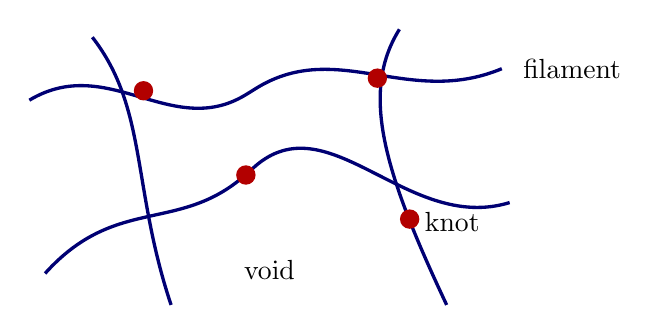
\begin{tikzpicture}[x=1cm,y=1cm]
  \draw[rounded corners=2pt,very thick,blue!45!black]
    (0.2,2.7) .. controls (1.2,3.3) and (2.0,2.2) .. (3.0,2.8)
    .. controls (4.1,3.5) and (5.0,2.6) .. (6.2,3.1);
  \draw[rounded corners=2pt,very thick,blue!45!black]
    (0.4,0.5) .. controls (1.3,1.5) and (2.1,1.0) .. (3.0,1.8)
    .. controls (4.0,2.7) and (5.0,1.0) .. (6.3,1.4);
  \draw[rounded corners=2pt,very thick,blue!45!black]
    (1.0,3.5) .. controls (1.7,2.6) and (1.5,1.6) .. (2.0,0.1);
  \draw[rounded corners=2pt,very thick,blue!45!black]
    (4.9,3.6) .. controls (4.4,2.8) and (4.7,1.8) .. (5.5,0.1);
  \fill[red!70!black] (1.65,2.82) circle (3.5pt);
  \fill[red!70!black] (4.62,2.98) circle (3.5pt);
  \fill[red!70!black] (2.95,1.75) circle (3.5pt);
  \fill[red!70!black] (5.03,1.19) circle (3.5pt);
  \node[align=center] at (3.25,0.55) {void};
  \node[right] at (6.35,3.1) {filament};
  \node[right] at (5.1,1.15) {knot};
\end{tikzpicture}
\caption{A clean two-dimensional analogy for the caustic network: line-like concentrations enclose voids and meet at brighter knots. In three dimensions the primary folds are sheets whose intersections form filaments and nodes.}
\label{fig:c09-caustic-network}
\end{figure}

The force-free construction is not a replacement for cosmological perturbation theory. Gravity is crucial to the growth of density contrast, halo formation, galaxies, and nonlinear structure. The toy model isolates one robust geometrical fact: a slightly varying initial flow naturally folds and concentrates. Small initial density variations could be included as well without changing the central Jacobian argument. \lecturetimestamp{02:06:49--02:07:34}

We have therefore moved the mystery rather than eliminated it. Inflation was introduced to stretch a region until it became extraordinarily flat and uniform. The caustic calculation assumes an initial field of tiny velocity variations. Where did that inhomogeneous seed come from? The next lecture turns to quantum fluctuations of fields during inflation and asks how they become the initial conditions for the later cosmic web. \lecturetimestamp{02:07:35--02:08:24}

\section{Summary}

A homogeneous scalar field behaves like a coordinate moving in the potential \(V(\phi)\). In a fixed box it obeys \(\ddot\phi=-V'(\phi)\). In an expanding comoving box, the physical volume \(a^3\) enters the action and produces
\[
\ddot\phi+3H\dot\phi=-V'(\phi).
\]
Hubble friction can hold the field to a slow terminal motion on a high, shallow potential. Its kinetic energy then becomes negligible, its potential energy keeps \(H\) nearly constant, and \(a(t)\) grows approximately exponentially.

That expansion dilutes unwanted monopoles, smooths geometry, and drives curvature toward zero. It must eventually end: the field leaves the plateau, oscillates, and transfers its energy into the hot particles of reheating. The shape of the potential, the identity and initial state of the inflaton, the reheating couplings, and the tiny present vacuum energy all remain open.

Inflation's success creates the final question. A perfectly smoothed universe would contain no galaxies. The caustic map
\[
y=x+v(x)t,
\qquad
\frac{dn}{dy}=\frac{1}{1+v'(x)t}
\]
shows how tiny variations in an initial flow can generate sharp sheets, filaments, and knots. It does not explain the origin of those variations. Their quantum origin is the subject to which the argument now turns.
